La section \ref{sec:prob} définit plus clairement la problématique à l'aide des éléments du chapitre précédent. Elle explique comment les différentes sections de ce chapitre confluent vers une solution à la problématique en question.

Ensuite, la section \ref{sec:fifo} étend le concept des automates aux automates à files et définit une nouvelle opération. Une forme de langage sur ces nouveaux automates est proposée à la section \ref{sec:trace}.

Finalement, la notion de sûreté est définie dans la section \ref{sec:unsafe} avec une formule permettant de calculer les états concernés.

Tous ces éléments combinés permettent l'utilisation de LeVer, la technique proposée par \cite{Vardhan04} et d'en implémenter l'algorithme dans le chapitre \ref{ch:impl}.



Cette section décrit le problème rencontré par \cite{Vardhan04} et la technique générale utilisée pour proposer une solution à ce problème.

Les automates à files définis à la section \ref{sec:fifo} sont plus puissants que les ADF définis dans le chapitre \ref{ch:bases}. Contrairement à ceux-ci, les automates à files ont potentiellement une infinité d'états. Dans ces conditions, il n'est pas possible d'en faire une exploration exhaustive pour trouver tous les états acceptants.

À la place, une propriété dite de sécurité est définie. Si un état respecte cette propriété, il est \emph{sécurisé}. Si il y a moyen de prouver que la totalité des états de l'automate respectent cette propriété, l'automate est considéré comme sécurisé. Si au contraire, un exemple de violation de la propriété est trouvé, l'automate peut être déclaré comme à risque.

Les sections suivantes donnent les différents éléments utilisés par \cite{Vardhan04} pour répondre à cette question. Un nouveau langage est donné pour représenter les différents états d'un automate à files. Celui-ci est construit pour pouvoir être régulier pour certains automates. De la sorte, il est possible d'appliquer l'algorithme d'Angluin pour apprendre ce nouveau langage.

Celui-ci n'étant qu'une approximation du langage de l'automate à files, certaines incertitudes peuvent apparaître. Cependant, l'article justifie ces différents cas en ramenant la question à la sécurité, qui peut être répondue en un temps polynomial.

Dès lors, les différentes sections permettent de construire ce langage, de se prononcer sur l'appartenance et l'équivalence avec ce langage et d'arrêter l'apprentissage s'il est possible de se prononcer sur la propriété de sécurité pour l'automate à files considéré.


\section{Approche}\label{app}Les automates à files définis à la section \ref{fifo} sont plus puissants que les ADF définis dans la section \ref{adf}. En effet, les systèmes de transitions associés ont potentiellement une infinité de configurations. Dans ces conditions, il n'est pas possible de faire une exploration exhaustive des états pour trouver lesquels sont acceptants.

À la place, une propriété dite de sécurité est définie. Si un état respecte cette propriété, il est \emph{sûr}. Si il y a moyen de prouver que la totalité des états de l'automate respectent cette propriété, l'automate est considéré comme sûr. Si au contraire, un exemple de violation de la propriété est trouvé, l'automate peut être déclaré comme à risque.

L'idée dès lors est de travailler non pas avec un système de transitions infini mais avec une représentation construite pour être finie dans un vaste ensemble de problèmes. Cette représentation est le langage de trace défini dans la section \ref{trace}.

En supposant que celui-ci est régulier, il est possible d'utiliser l'algorithme d'Angluin de la section \ref{angluin} pour l'apprendre. Cependant, ce langage n'est qu'un concept et le professeur n'a accès qu'à un automate à files $F$. Pour cette raison, les oracles d'appartenance et d'équivalence sont adaptés pour répondre à une requête entre un langage fourni par l'élève et $F$.

La figure \ref{fig:lever} donne une vue schématique de ce nouvel algorithme d'Angluin modifié.


\begin{figure}[H]
	\centering

	\resizebox{\textwidth}{!}{
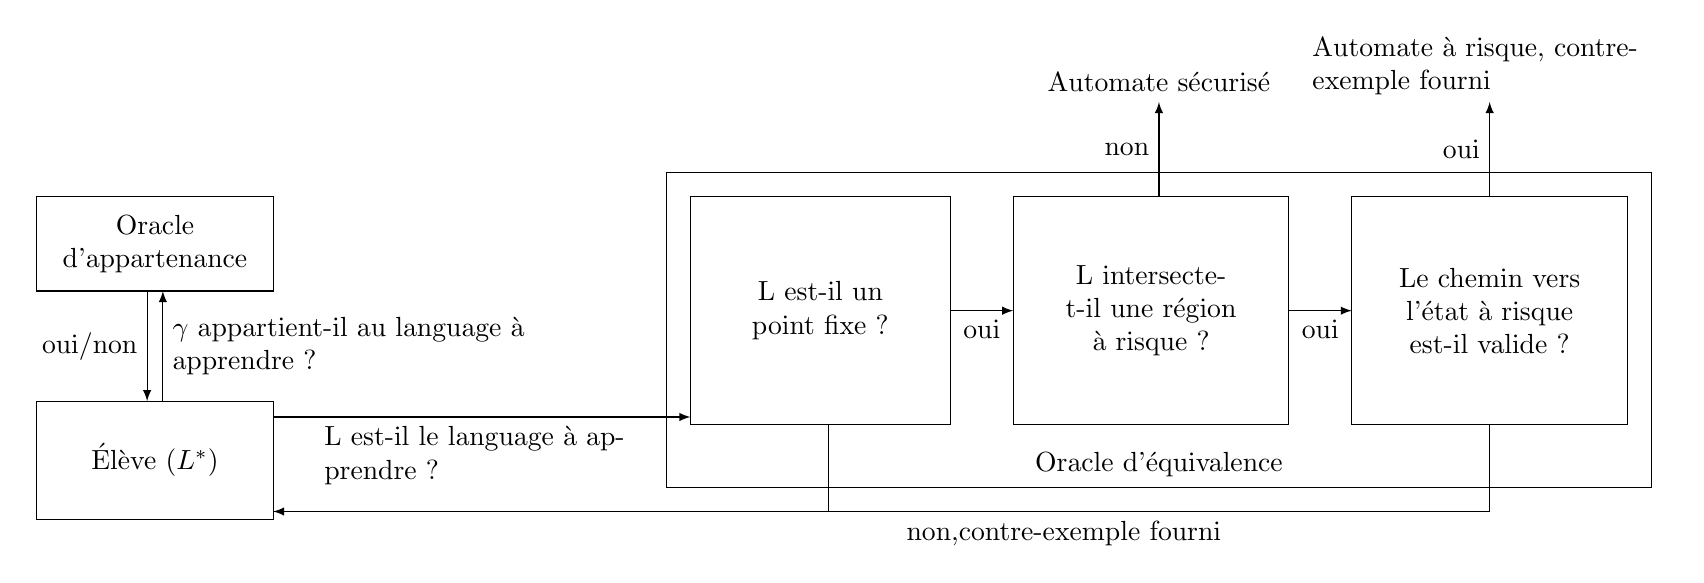
\begin{tikzpicture}
	\tikzset{>=latex}

  \draw (-3,-2.9) rectangle (0,-4.4) node[pos=.5] {Élève ($L^*$)};
  \draw (5,0) rectangle (17.5,-4);
	\draw[->] (0,-3.1) -- (5.3,-3.1) node[pos=0.5,below,text width=4cm] {L est-il le language à apprendre ?};

  \draw (-3,-0.3) rectangle (0,-1.5) node[pos=.5,text width=3cm,align=center] {Oracle\\ d'appartenance};
  \draw[->] (-1.4,-2.9) -- (-1.4,-1.5) node[pos=0.5,right,text width=5cm] {$\gamma$ appartient-il au language à apprendre ?};
  \draw[<-] (-1.6,-2.9) -- (-1.6,-1.5) node[pos=0.5,left] {oui/non};

  \node[draw=none] at (11.25, -3.7) {Oracle d'équivalence};

  \draw (5.3, -0.3) rectangle (8.6, -3.2) node[pos=0.5,text width=3cm,align=center] {L est-il un point fixe ?};
  \draw (9.4, -0.3) rectangle (12.9, -3.2) node[pos=0.5,text width=3cm,align=center] {L intersecte-t-il une région à risque ?};
  \draw (13.7, -0.3) rectangle (17.2, -3.2) node[pos=0.5,text width=3cm,align=center] {Le chemin vers l'état à risque est-il valide ?};

  \draw[->] (8.6, -1.75) -- (9.4,-1.75) node[pos=0.5,below] {oui};
  \draw[->] (12.9, -1.75) -- (13.7,-1.75) node[pos=0.5,below] {oui};
  \draw[->] (15.45, -4.3) -- (0, -4.3) node[pos=0.35,below] {non,contre-exemple fourni};
  \draw[-] (7.05, -3.2) -- (7.05, -4.3);
  \draw[-] (15.45, -3.2) -- (15.45, -4.3);

	\draw[->] (11.25,-0.3) -- (11.25,0.9)node[pos=0.5,left] {non};
	\draw[->] (15.45,-0.3) -- (15.45,0.9)node[pos=0.5,left] {oui};

	\node[draw=none] at (11.25, 1.15) {Automate sécurisé};
	\node[draw=none,text width=4.5cm] at (15.45, 1.36) {Automate à risque, contre-exemple fourni};


\end{tikzpicture}
}
\caption{Vue schématique de l'algorithme d'Angluin pour LeVer\cite{Vardhan04}}\label{fig:lever}
\end{figure}


\emph{LeVer} est le nom de cette technique. En particulier, on peut noter sur ce schéma que l'oracle d'équivalence peut non seulement répondre oui ou non mais également interrompre l'apprentissage s'il est possible de se prononcer sur la sûreté d'un automate à files $F$. Pour rappel, $L(F)$ n'est pas régulier en général. Pouvoir se prononcer sur la sûreté de $F$ étant possible, il n'est ni utile ni forcémment possible de continuer à appliquer $L^*$ pour obtenir une meilleure approximation $L$ du langage de trace de $F$. 

\section{Langage de trace}\label{trace}Cette section s'intéresse aux langages qui peuvent être associés à un automate. La section \ref{ss:trace} défini le langage de trace d'un automate. Celui-ci n'est pas nécessairement régulier. Les sections suivantes s'appuyent sur \cite{Vardhan04} pour proposer un langage régulier qui représente ce langage de trace.


% ██       █████  ███    ██  ██████
% ██      ██   ██ ████   ██ ██
% ██      ███████ ██ ██  ██ ██   ███
% ██      ██   ██ ██  ██ ██ ██    ██
% ███████ ██   ██ ██   ████  ██████

\subsection{Langage tracé}\label{ss:trace}

Une façon de définir un langage à partir d'un automate FIFO est de s'intéresser aux noms des transitions suivies lors de l'exécution. Cette section défini les éléments permettant d'arriver à la construction d'un tel langage.

Dans un système de transitions \tsys, la fonction de transition $\rightarrow:S\times\Theta\rightarrow S$ permet de définir le passage d'un état à un autre.

La \emph{fonction de transition étendue} $\xrightarrow{*}$ est la fermeture transitive et réflexive de $\rightarrow$.

Pour une suite de noms de transitions $\sigma=\theta_1\theta_2 ...\theta_n\in\Theta^*$, on note $(p,w)\xrightarrow{\sigma}(q,w')$ si il existe des états $(p_1,w_1)(p_2,w_2)...(p_{n-1},w_{n-1})$ tels que $(p,w)\xrightarrow{\theta_1}(p_1,w_1)\xrightarrow{\theta_2}...\xrightarrow{\theta_{n-1}}(p_{n-1},w_{n-1})\xrightarrow{\theta_n}(q,w')$. Dans ce cas, $\sigma$ est une \emph{trace de chemin}.

\begin{definition} Soit un automate FIFO $F$ et l'état initial $s_0=(q_0, \epsilon^C)$. Celui-ci est le couple état de contrôle initial $q_0$ ainsi que des mots $w[c]=\epsilon$ pour tout canal $c\in C$.

  Le \emph{langage de trace} d'un automate $F$ est

  $$
  L(F)=\{\sigma\in\Theta^*|\exists s=(p,w) \text{ tel quel } s_0\xrightarrow{\sigma}s\}
  $$
\end{definition}

\begin{example}
  Considérons l'automate FIFO $F$ de la figure \ref{fig:fifo1}.

  Pour celui-ci, $\sigma=\theta_1\theta_4\theta_7$ n'est pas un chemin. En effet,
  $$
  (q_0,[\epsilon,\epsilon])\xrightarrow{\theta_1}(q_1,[0,\epsilon])\xrightarrow{\theta_4}(q_3,[\epsilon,\epsilon])
  $$

  Mais, il n'existe pas d'état $s$ tel que $(q_3,[\epsilon,\epsilon])\xrightarrow{\theta_7}s$. En effet, pour appliquer cette transition, il aurait fallu que le canal $b$ contienne un symbole $0$. Ce n'est pas le cas.


  Par contre, $\sigma=\theta_2\theta_5\theta_5\theta_6\theta_7\theta_1\theta_4\theta_7$ est un chemin dans $F$ :
  \begin{equation*}
    \begin{gathered}
      (q_0,[\epsilon,\epsilon])\xrightarrow{\theta_2}
      (q_0,[1,\epsilon])\xrightarrow{\theta_5}
      (q_0,[1,0])\xrightarrow{\theta_5}
      (q_0,[1,00])\xrightarrow{\theta_6}
      (q_0,[\epsilon,00])\xrightarrow{\theta_7}\\
      (q_0,[\epsilon,0])\xrightarrow{\theta_1}
      (q_0,[0,0])\xrightarrow{\theta_4}
      (q_0,[\epsilon,0])\xrightarrow{\theta_7}
      (q_0,[\epsilon,\epsilon])
    \end{gathered}
  \end{equation*}

  On a bien un état $s$ (ici $s=(q_0,[\epsilon,\epsilon])=s_0$) tel que $s_0\xrightarrow{\sigma}s$.

\end{example}

  % ████████ ██   ██ ███████ ████████  █████
  %    ██    ██   ██ ██         ██    ██   ██
  %    ██    ███████ █████      ██    ███████
  %    ██    ██   ██ ██         ██    ██   ██
  %    ██    ██   ██ ███████    ██    ██   ██



\subsection{Alphabet d'annotation}

Le langage de trace n'est pas nécessairement régulier. Pour permettre l'apprentissage par l'algorithme d'Angluin, il faut en construire un qui est régulier et qui permette de reconstruire le langage de trace. Pour ce faire, ce nouveau langage devrait pouvoir représenter tout état atteignable ainsi qu'un ou plusieurs chemins ou mots témoins permettant d'atteindre ceux-ci.

Pour ce faire, pour chaque nom de transition correspondant à une action d'envoi, un \emph{co-nom} est défini :
$$
\bar{\Theta}=\{\bar{\theta}|\theta\in\Theta\wedge\exists p,q \in Q, c\in C, a\in\Sigma,\text{tels que } \delta(\theta)=(p,c!a,q)\}
$$

De plus, un \emph{symbole de contrôle} est créé pour chaque état de contrôle : $T_Q = \{t_q | q\in Q\}$.

En combinant les noms de transitions, les co-noms et les symboles de contrôlé, un nouvel alphabet peut-être défini, l'\emph{alphabet d'annotation} : $\Phi=(\Theta-\Theta_r)\bigcup\bar{\Theta}\bigcup T_Q$.

Avec $\Theta_r=\{\theta|\theta\in\Theta\wedge\exists p,q \in Q, c\in C, a\in\Sigma,\text{tels que } \delta(\theta)=(p,c?a,q)\}$, similaire à $\bar{\Theta}$ mais avec un nom pour chaque transition pour les actions de réception.


\subsection{Trace annotée}


Soit $\mathcal{A}:\Theta^*\rightarrow\Phi^*$ une fonction associant une \emph{trace annotée} à une trace d'automate. Cette fonction est décrite par l'algorithme \ref{alg:A}.


\begin{algorithm}[H]
  	\begin{algorithmic}[1]
    \REQUIRE un automate FIFO \fifo , une suite de noms de transitions $\sigma\in\Theta^*$
		\ENSURE une trace annotée $\gamma\in\Phi^*$ représentant $\sigma$

    \STATE $\gamma\leftarrow\epsilon$
    \FORALL {transition $\theta\in\sigma$}
      \IF {$\theta$ correspond à une action de réception}
        \STATE trouver $\theta_s\in\Theta$ correspondant à une action d'envoi antécédant dans $\sigma$ tel que les actions s'appliquent sur le même canal et le même symbole
        \STATE $\gamma\leftarrow$ $\gamma$ où $\theta_s$ est remplacé par $\bar{\theta_s}\in\bar{\Theta}$ \COMMENT {$\theta$ n'est pas ajouté à $\gamma$}
      \ELSIF {$\theta$ correspond à une action d'envoi}
        \STATE $\gamma\leftarrow\gamma\theta$
      \ENDIF
    \ENDFOR
    \STATE trouver $q$ l'état de contrôle tel que $\delta(\theta)=(p,a,q)$ avec $p\in Q,a\in((C \times \{?,!\} \times \Sigma) \bigcup \{\tau\})$
    \STATE $\gamma\leftarrow\gamma t_q$ avec $t_q\in T_Q$ le symbole de contrôle associé à $q$
		\RETURN $\gamma$
	\end{algorithmic}
	\caption{$\mathcal{A}:\Theta^*\rightarrow\Phi^*$}\label{alg:A}
\end{algorithm}

Soit $AL(F)=\{\mathcal{A}(\sigma)|\sigma \in L(F)\}$ le \emph{langage de traces annotées} de l'automate $F$. $AL(F)$ est un ensemble de traces annotées correspondant à des exécutions valides de l'automate $F$. Intuitivement, $AL(F)$ contient l'ensemble des états atteignables par $F$ ainsi que les traces annotées servant de témoins de cette atteignabilité des états.


Soit un mot $\gamma \in \Phi^*$. $\gamma$ est \emph{correctement formaté} si il fini par un symbole de $T_Q$ qui qu'aucun autre symbole de cet ensemble n'apparaît dans le mot. Soit un langage arbitraire $L$. $L$ est \emph{correctement formaté} si tous les mots de $L$ le sont.


\begin{example}
Soit l'automate $F$ représenté par la figure \ref{fig:fifoAB}. Soient les séquences $\sigma_1=\theta_2\theta_8$ et $\sigma_2=\theta_1\theta_3\theta_5\theta_2$. Alors, les traces annotées de ces traces sont : $\mathcal{A}(\sigma_1)=\theta_2\theta_8t_{(q_1,q_B)}=\gamma_1$ et $\mathcal{A}(\sigma_2)=\bar{\theta_1}\bar{\theta_5}t_{(q_0,q_B)}=\gamma_2$.
Bien qu'elles soient toutes deux correctement formatées, $\gamma_1$ ne correspond à aucune exécution valide de $F$. Dès lors, $\gamma_1$ n'appartient pas au langage de traces annotées de $AL(F)$ contrairement à $\gamma_2$.

Soit le mot $\gamma_3=t_{q_0,q_A}\theta_2 t_{q_0,q_B} \in \Phi^*$. $\gamma_3$ n'est pas correctement formaté : il est impossible que ce mot appartienne à $AL(F)$.
\end{example}

\section{Appartenance}\label{mem}Lorsqu'un mot $\gamma$ est fourni à l'oracle d'appartenance la question est de savoir s'il apparatient à $AL(F)$, le langage de trace annotée. Comme l'oracle ne possède pas d'automate pour représenter ce langage, il doit répondre en se basant sur $F$.

Ainsi donc, un mot $\gamma$ appartient à $AL(F)$ s'il représente au moins un chemin $\theta$ valide dans $F$.

Soit une fonction $\mathcal{A}^{-1}(\gamma)$ donnant l'ensemble des chemins $\theta$ pour lesquels $\mathcal{A}(\theta)=\gamma$. Si $\mathcal{A}^{-1}(\gamma)\neq\emptyset$, c'est que $\gamma$ correspond bien à un chemin dans $F$; que $\gamma\in AL(F)$.

Premièrement, si $\gamma$ est incorrectement formaté, $\mathcal{A^{-1}}(\gamma)=\emptyset$ puisque tout mot de $AL(F)$ est conforme par définition.

Supposant que $\gamma$ est correctement formaté, on peut remplacer les symboles barrés (appartenant à \barTheta) par leur équivalent non barré (de $\Theta$). De plus, l'état final est omis. De la sorte, on obtient un mot $\theta'$ qui pourrait appartenir à $\mathcal{A}^{-1}$ si les transitions de réceptions correspondant aux états d'envois qui étaient barrés n'étaient pas omises.

Il est possible d'identifier ces transitions de réception. Dans le corps de $\gamma$, chaque envoi barré peut être associé à une transition de réception sur le même canal pour le même symbole. Cependant, la position à laquelle insérer de telles transitions dans le mot est inconnue.

Pour ce faire, il est possible de tester toutes les différentes positions (qui est un ensemble fini), et tester celles-ci sur l'automate $F$. Dès lors, toute séquence $\theta$ valide pour laquelle $\mathcal{A}(\theta)=\gamma$ appartient à $\mathcal{A}^{-1}(\gamma)$, rendant l'ensemble non-vide. Une seule séquence est suffisante pour garantir que $\gamma\in AL(F)$.

\begin{example}
Considérons l'automate \ref{fig:fifoA}. Pour rappel, celui-ci comprend trois transitions ($\delta(\theta_1)=(q_0, a!1, q_1)$, $\delta(\theta_2)=(q_1,a?1,q_2)$, et $\delta(\theta_3)=(q_2, a!0, q_0)$).

Une trace annotée $\gamma=\bar{\theta_1}\theta_3\theta_1q_1$ appartient bien à $AL(A)$. En effet, $\mathcal{A}^-1(\gamma)=\{\theta_1\theta_2\theta_3\theta_1\}$.

Par contre, la trace $\gamma=\bar{\theta_1}\bar{\theta_1}\theta_3q_0$ ne convient pas. Aucun chemin $\theta$ ne permet $\mathcal{A}(\theta)=\gamma$. Il est facile de s'en convaincre : le chemin passe deux fois par $\theta_1$ sans passer par $\theta_3$ qui est ici inévitable pour retourner à l'état de contrôle $q_0$.

\end{example}

\section{Équivalence}\label{eq}Lorsqu'un langage régulier $L$, représenté par un automate $A_O$ tel que $L(A_O)=L$, est donné à l'oracle d'équivalence, il doit se prononcer sur $L=AL(F)$. Cependant, il ne possède pas d'automate pour $AL(F)$ qui est justement le langage recherché. Il doit alors se prononcer sur l'égalité en se basant uniquement sur $F$.

Comme expliqué dans l'introduction du chapitre, c'est impossible de façon générale. Cependant, en supposant que $AL(F)$ est régulier, il est possible de contourner le problème pour répondre à la question de sécurité.

Contrairement à la version originale de l'algorithme d'Angluin qui a deux possibilités (équivalence ou contre-exemple), celle-ci en a trois. L'oracle peut répondre soit que $AL(F)$ est sécurisé, soit qu'il ne l'est pas, soit que $L$ est différent de $AL(F)$ avec un contre-exemple.


\subsection{$L$ est-il un point fixe de $\mathcal{F}$ ?}\label{ss:fixe}

Cette question se base sur le théorème \ref{thm:fl} et en particulier du fait que $AL(F)$ est un point fixe. Il n'est pas possible de prouver que $L=AL(F)$ mais il est possible de montrer que $L\neq AL(F)$ en montrant que $L$ n'est pas un point fixe.

Une façon de montrer que $L\neq AL(F)$, est d'énoncer un seul élément dans $L\bigcup AL(F)-L\bigcap AL(F)=$\alfx, \emph{l'union exclusive} des deux ensembles. Pour rappel, $AL(F)$ est un langage contenant l'ensemble des traces valides pour l'automate à files $F$.

En comparant \fl avec $L$ pour vérifier si $L$ est un point fixe de $\mathcal{F}$, plusieurs situations peuvent apparaître :

\begin{itemize}
  \item $\mathcal{F}(L)-L\neq\emptyset$. Considérons une trace annotée $\gamma\in\mathcal{F}(L)-L$ et montrons que $\gamma\in$\alfx.
  \begin{itemize}
    \item Si $\gamma=t_{q_0}$, c'est que $t_{q_0}\notin L$. Pourtant, par définition, $t_{q_0}\in AL(F)$. Dès lors, $\gamma\in$\alfx
    \item Sinon, si $\gamma$ est une annotation valide, c'est que $L$ n'est pas un point fixe de $\mathcal{F}$. Dès lors, $\gamma$ suffit à démontrer que $AL(F)\neq L$.
    \item Sinon, $w$ n'est pas une annotation valide. $\gamma$ faisant partie de \fl, cela signifie qu'il doit exister une trace annotée $\gamma'\in L$ telle que $\gamma=Post(\gamma')$. Ce $\gamma'$ ne peut pas être une annotation valide : cela impliquerait que $\gamma$ l'est également ce qui est posé comme faux ici. Comme $\gamma'$ n'est pas une annotation valide pour $F$, $\gamma'\notin AL(F)$. Comme $\gamma'\in L$, naturellement $\gamma'\in$\alfx.
  \end{itemize}
  \item $\mathcal{F}(L)\subsetneq L$. Dans ce cas, utilisons la notion de point préfixe. Un ensemble $Z$ est un \emph{point préfixe} d'une fonction $\mathcal{F}$ s'il réduit par son application : $\mathcal{F}$ ($\mathcal{F}(Z)\subseteq Z$). Selon cette définition, $L$ est un point préfixe de $\mathcal{F}$.
  En appliquant $\mathcal{F}$ des deux côtés, ce qui préserve l'inclusion car $\mathcal{F}$ est monotone, on obtient $\mathcal{F}(\mathcal{F}(L))\subsetneq\mathcal{F}(L)$.

  Donc, $\mathcal{F}(L)$ est également un point préfixe. Soit $\gamma\in L-\mathcal{F}(L)$. Comme $\gamma$ n'est pas dans l'intersection de ces deux point préfixes, il ne fait pas partie du point fixe minimum $AL(F)$. En effet, selon la théorie des points fixes de Knaster-Tarski (annexe \ref{app:tarski}), un point fixe minimal est également l'intersection de tous les points préfixes de $\mathcal{F}$.

  \item \fl=$L$. Cela signifie que $L$ est un point fixe de $\mathcal{F}$. Cela signifie qu'il n'est pas possible de prouver que $L\neq AL(F)$ et infirmant cette propriété. Cela ne signifie par pour autant que $L=AL(F)$.

  Ce pourrait très bien être un autre point fixe contenant $AL(F)$ ou un autre ensemble contenant une trace annotée menant à un état qui n'est pas sûr. Pour tenter de continuer à chercher un contre-exemple ou tester la sûreté, il faut poser d'autres questions.

\end{itemize}

La transcription en algorithme de la comparaison entre $L$ et $\mathcal{F}(L)$ pour trouver un contre-exemple à $L=AL(F)$ est donnée dans la section \ref{sec:fll}, accompagnée d'un exemple.


\subsection{$L$ intersecte-t-il avec une région à risque ?}

En visualisant $L$ comme étant un super-ensemble de $AL(F)$ et la région à risque comme un ensemble, il est possible de se représenter les différentes situations envisageables.

\begin{figure}[H]

  \colorlet{circle edge}{black}
  \colorlet{circle area}{blue!20}
  \colorlet{circle darker}{blue!40}
  \tikzset{filled/.style={fill=circle area, draw=circle edge},
    outline/.style={draw=circle edge}}

  \def\circleL{ (0,0) circle (1.5cm) node[right=0.8cm]  {$L$}}
  \def\circleAL{(-0.15,-0.3) circle (1cm) node {$AL(F)$}}

 \centering
 \begin{subfigure}{0.33\textwidth}
  \centering
  \def\circleUS{(0,2.8) circle (1cm) node[text width=1.5cm,align=center]  {Région à risque}}
  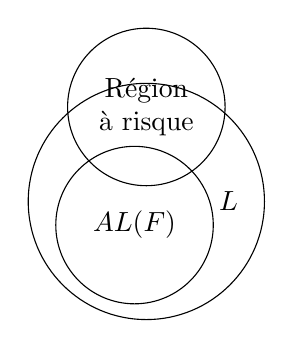
\begin{tikzpicture}
   \draw[outline]\circleL;
   \draw[outline]\circleAL;
   \draw[outline]\circleUS;
  \end{tikzpicture}
  \caption{Pas d'intersection}
 \end{subfigure}%
 \begin{subfigure}{0.33\textwidth}
  \centering
  \def\circleUS{(0,2.2) circle (1cm) node[text width=1.5cm,align=center]  {Région à risque}}
  \vspace{0.6cm}
  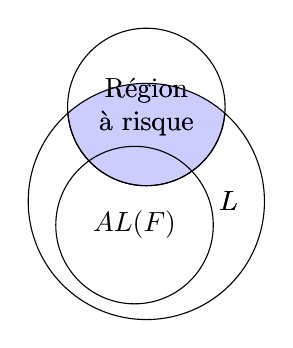
\begin{tikzpicture}
    \begin{scope}
        \clip \circleL;
        \fill[filled] \circleUS;
    \end{scope}
    \draw[outline]\circleL;
    \draw[outline]\circleAL;
    \draw[outline]\circleUS;
  \end{tikzpicture}
  \caption{Intersection avec $L$ seulement}
 \end{subfigure}
 \begin{subfigure}{0.33\textwidth}
   \centering
   \def\circleUS{(0,1.2) circle (1cm) node[text width=1.5cm,align=center]  {Région à risque}}
   \vspace{1.6cm}
   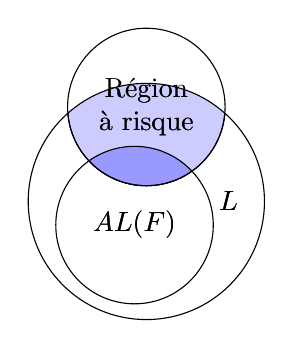
\begin{tikzpicture}
     \begin{scope}
         \clip \circleL;
         \fill[filled] \circleUS;
     \end{scope}
     \begin{scope}
         \clip \circleAL;
         \fill[filled, fill=circle darker] \circleUS;
     \end{scope}
     \draw[outline]\circleL;
     \draw[outline]\circleAL;
     \draw[outline]\circleUS;
   \end{tikzpicture}
  \caption{Intersection avec $AL(F)$}
 \end{subfigure}
 \caption{$L$, $AL(F)$ et la région à risque}\label{fig:inter}
\end{figure}

Pour savoir si nous sommes dans le scénario (a), (b) ou (c) de la figure \ref{fig:inter}, deux tests sont à effectuer.

Premièrement, vérifier si l'intersection avec la région à risque $\mathcal{W}(L)$ est vide ou non. S'il est vide, nous sommes dans le scénario (a) et il est possible d'annoncer avec certitude que $F$ est sécurisé.

\subsection{Le chemin vers l'état à risque est-il valide ?}

Si la réponse à la question précédente est oui, sommes-nous dans le scénario (b) ou (c) ?
Considérons un des éléments de $\mathcal{W}(L)$. Demandons à l'oracle d'appartenance si ce mot appartient également à $AL(F)$.

Si ce n'est pas le cas, c'est que $L\neq AL(F)$ et que l'algorithme d'Angluin peut continuer grâce au contre-exemple fourni. Ici, il peut s'agir soit d'un scénario (b) soit d'un scénario (c) puisqu'un autre mot de $\mathcal{W}(L)$ pourrait appartenir à $AL(F)$. Cela correspondrait à prendre un mot de la zone bleue claire dans (c).

Améliorer l'approximation d'$AL(F)$ permet justement de mieux discerner ces deux scénarios sans devoir consulter la totalité de $\mathcal{W}(L)$.

Si par contre le mot étudié appartient aussi à $AL(F)$, on a un mot étant à la fois dans $AL(F)$ et dans la région à risque. $F$ est déclaré à risque et le mot est retourné comme contre-exemple. Il s'agit du scénario (c).

\section{Sûreté}\label{safety}Comme mentionné au début du chapitre, ce travail s'intéresse à la propriété de unsafe dans les automates FIFO. Contrairement aux ADF construits dans le chapitre \ref{ch:bases}, les automates FIFO ont un nombre potentiellement infini d'états. Dans ces conditions, il n'est pas possible d'énumérer l'ensemble des états acceptants.

Au lieu de proposer un ensemble d'état acceptants, on va fixer une propriété. Si un état respecte cette propriété, il est dit safe. Il est donc unsafe s'il ne respecte pas cette propriété de safety. Par la suite, la section \ref{ss:tracesafety} propose une technique permettant de calculer les états unsafe pour un langage de traces annotées. Ceci permet de répondre à la question de safety directement depuis ce langage au lieu de devoir construire le langage de l'automate FIFO.


\subsection{Définition}
Dans un automate FIFO \fifo, chaque état de contrôle $q\in Q$ est associé à un union finie de langage réguliers pour chacun des canaux $c\in C$.


$$\bigcup_{0 \leq i \leq n_q}\Pi_{0 \leq j \leq k}U_q(i,c_j)$$

Où $U_q(i,c_j)$ est un langage régulier pour le contenu du canal $c_j$ sur l'état $q$. $n_q$ est le nombre de langages réguliers utilisés pour définir cette propriété par union.

Un état $s=(q,[w_0,w_1,\dots,w_k])$ est \emph{unsafe} s'il existe $i,j \in \mathcal{N}$ tels que $w_j \in U_q(i,c_j)$.



\subsection{Traces annotées menant à des états unsafe}\label{ss:tracesafety}




$$
W(L)=\bigcup_{q\in Q}\big(\bigcup_{0\leq i\leq n_q}\big(\bigcap_{0\leq j \leq k}h_{c_j}^{-1}(U_q(i,c_j))\big)\big)
$$


\begin{theorem}
  Pour vérifier la propriété de safety des automates FIFO, l'algorithme LeVer respecte les propriétés suivantes :
  \begin{enumerate}
    \item Si l'algorithme retourne une réponse, celle-ci est correcte
    \item Si $AL(F)$ est régulier, la procédure s'arrête.
    \item Le nombre de test d'appartenance et d'éuivalence dépend principalement de l'algorithme d'Angluin. Le temps total est borné en temps polynomial du nombre d'états de l'automate minimal pour $AL(F)$ et linéaire en le temps pris pour une requête d'appartenance à $AL(F)$
  \end{enumerate}
\end{theorem}

La preuve est disponible en annexe du document \cite{Vardhan04} mais c'est un résultat tellement important, il est peut-être pertinent que celle-ci soit rediscutée ici.

\section{Algorithme}\label{lever}Dans les chapitres précédants, les bases théoriques sur les automates et languages ont été introduites. Celles-ci ont été suivies de concepts plus étroitement liés à LeVer tels que les automates à files, les traces, traces annotées et languages associés. Un dernier élément présenté dans la section \ref{sec:unsafe} est la sécurité d'un état ou d'un automate.

En appliquant l'algorithme d'Angluin \cite{Angluin87} selon la méthode LeVer \cite{Vardhan04}, il est possible de se prononcer sur la sécurité pour toute une classe d'automates à files : ceux pour lesquels le language de traces annotées est régulier.

L'objectif dès lors n'est pas d'apprendre le language de l'automate à file mais le language de trace associé, et d'adapter la méthode pour répondre à la question de sécurité. En formulant les bonnes propriétés, il est également possible d'interrompre l'algorithme d'apprentissage avant terme si l'on peut se prononcer sur la sécurité de façon certaine.


\begin{figure}[H]
	\centering

	\resizebox{\textwidth}{!}{
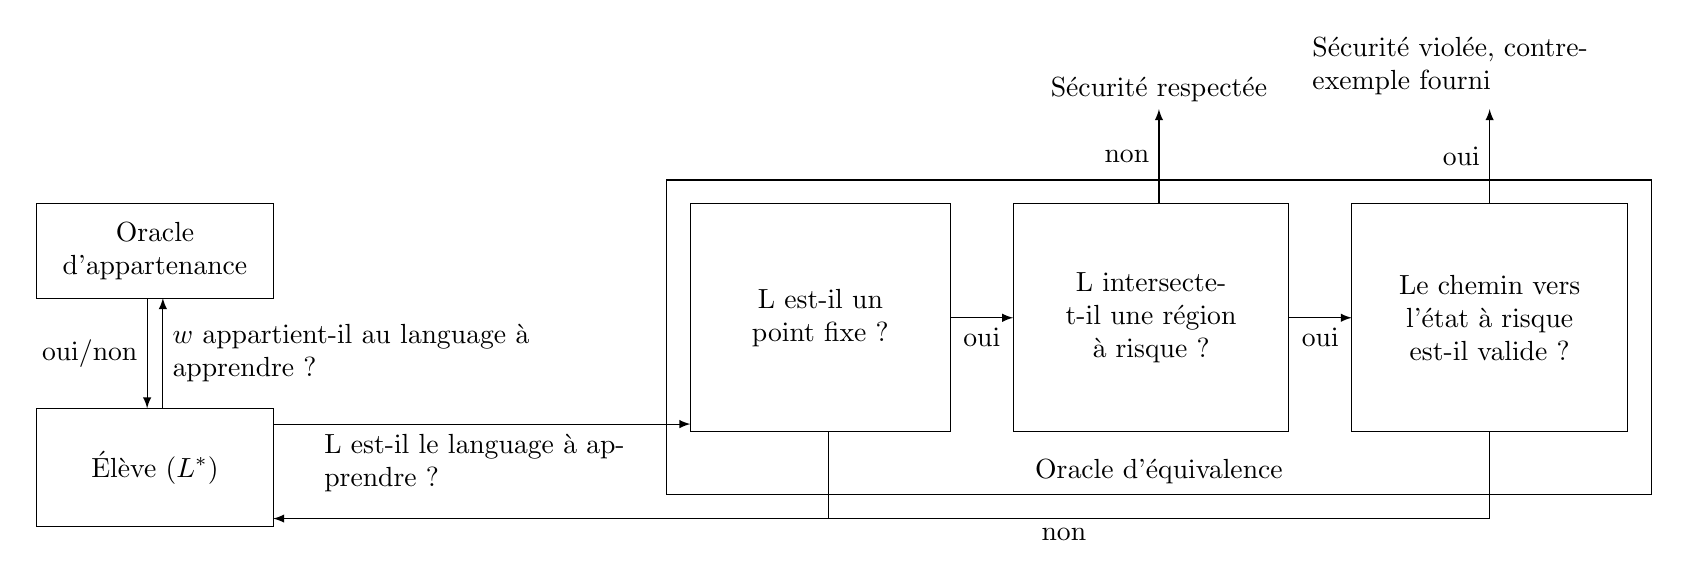
\begin{tikzpicture}
	\tikzset{>=latex}

  \draw (-3,-2.9) rectangle (0,-4.4) node[pos=.5] {Élève ($L^*$)};
  \draw (5,0) rectangle (17.5,-4);
	\draw[->] (0,-3.1) -- (5.3,-3.1) node[pos=0.5,below,text width=4cm] {L est-il le language à apprendre ?};

  \draw (-3,-0.3) rectangle (0,-1.5) node[pos=.5,text width=3cm,align=center] {Oracle\\ d'appartenance};
  \draw[->] (-1.4,-2.9) -- (-1.4,-1.5) node[pos=0.5,right,text width=5cm] {$w$ appartient-il au language à apprendre ?};
  \draw[<-] (-1.6,-2.9) -- (-1.6,-1.5) node[pos=0.5,left] {oui/non};

  \node[draw=none] at (11.25, -3.7) {Oracle d'équivalence};

  \draw (5.3, -0.3) rectangle (8.6, -3.2) node[pos=0.5,text width=3cm,align=center] {L est-il un point fixe ?};
  \draw (9.4, -0.3) rectangle (12.9, -3.2) node[pos=0.5,text width=3cm,align=center] {L intersecte-t-il une région à risque ?};
  \draw (13.7, -0.3) rectangle (17.2, -3.2) node[pos=0.5,text width=3cm,align=center] {Le chemin vers l'état à risque est-il valide ?};

  \draw[->] (8.6, -1.75) -- (9.4,-1.75) node[pos=0.5,below] {oui};
  \draw[->] (12.9, -1.75) -- (13.7,-1.75) node[pos=0.5,below] {oui};
  \draw[->] (15.45, -4.3) -- (0, -4.3) node[pos=0.35,below] {non};
  \draw[-] (7.05, -3.2) -- (7.05, -4.3);
  \draw[-] (15.45, -3.2) -- (15.45, -4.3);

	\draw[->] (11.25,-0.3) -- (11.25,0.9)node[pos=0.5,left] {non};
	\draw[->] (15.45,-0.3) -- (15.45,0.9)node[pos=0.5,left] {oui};

	\node[draw=none] at (11.25, 1.15) {Sécurité respectée};
	\node[draw=none,text width=4.5cm] at (15.45, 1.45) {Sécurité violée, contre-exemple fourni};


\end{tikzpicture}
}
\caption{Vue schématique de l'algorithme d'Angluin pour LeVer\cite{Vardhan04}}

\end{figure}


\todo{Ce chapitre décrit le fonctionnement de LeVer en se basant sur tout le reste. Concrètement, il s'agit d'une reformulation de l'algorithme d'Angluin pour les automates FIFO selon la méthode de Vardhan}

\todo{Cette section explique le but recherché, son importance et la structure du chapitre}

